\subsection{Bayesian Inference} \label{BaysRes}
The Bayesian inversion approach samples a posterior distribution of depth profiles. For comparison to the other inversion methods, we consider only the depth at each grid point which corresponds to the maximum of the posterior probability distribution at that point. This is achieved by taking the maximum of the kernel density of the estimated depth distribution at each point along the 1D profile. 

\subsubsection{Manufactured Data Result}
This method is first applied to the synthetic data $\mathbf{k}_s$ and the resulting depth estimate is shown in Figure~\ref{mcmc-synthetic}. As for other methods, the synthetic result accurately represents the sandbar located at x position$~\sim950~m$ along the profile, which is an important feature to recreate. However, at offshore locations (x position$<600~m$), the estimation appears to break down. As in other methods, this is expected because of the lower sensitivity of $k$ on $h$ at these depths, a relationship on which our inverse methods rely.

\begin{figure}[H]
\center
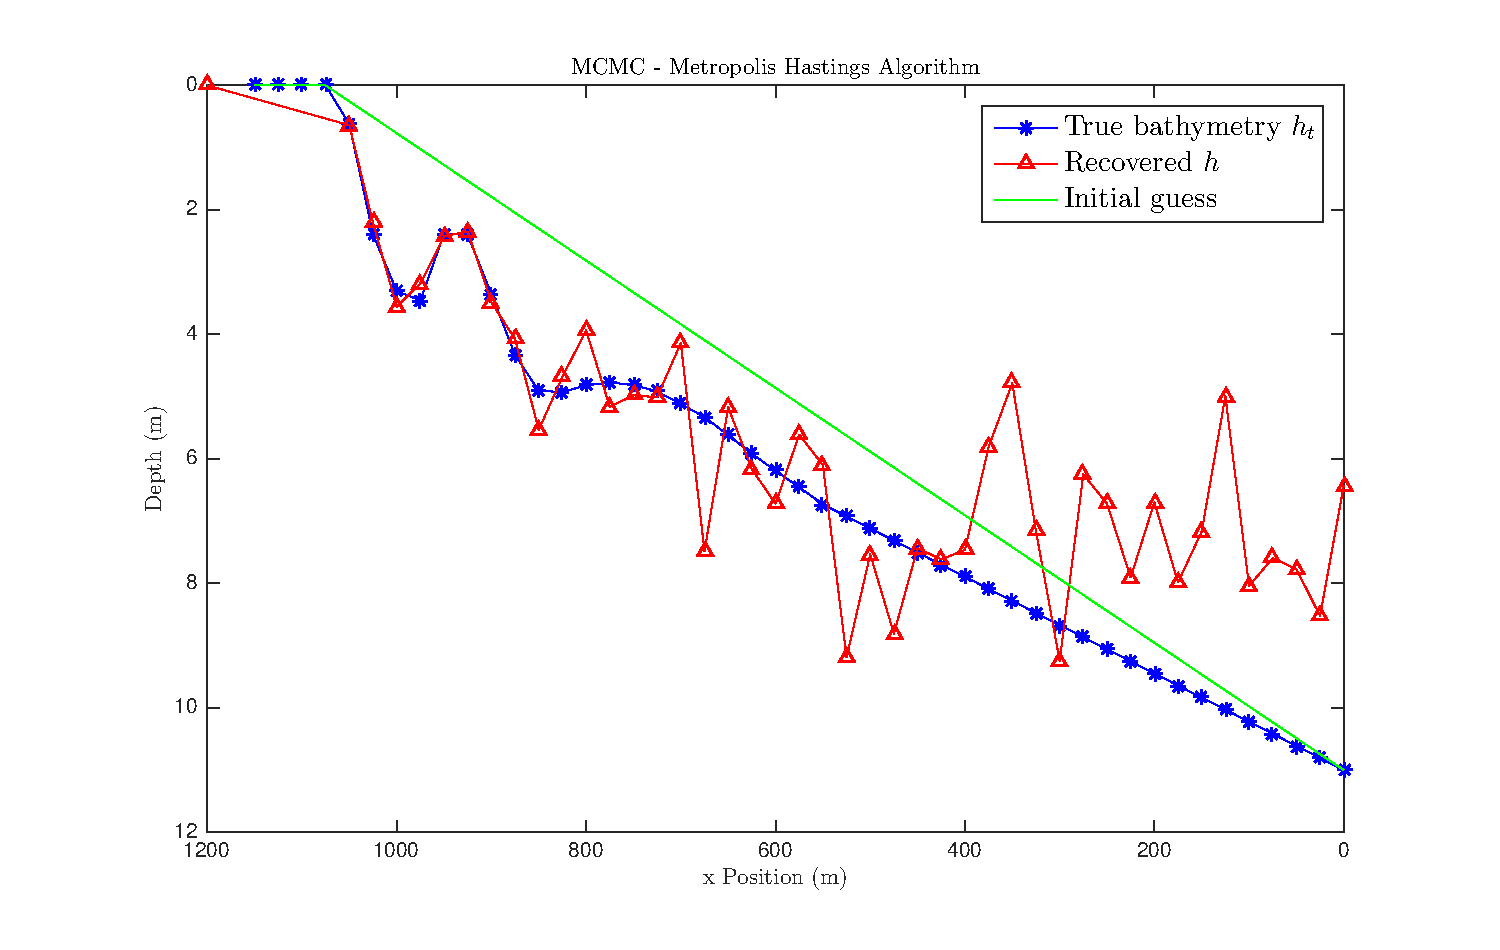
\includegraphics[scale=0.46]{img/MCMC-manufactured.eps} 
\caption{Bathymetry estimate from the Bayesian Markov Chain Monte Carlo (MCMC) approach using the synthetic wave numbers with 25m grid resolution. The initial depth guess is shown in green, the true depth is shown in blue, and the derived estimate of depth is shown in red.}
\label{mcmc-synthetic}
\end{figure}

The Markov Chain Monte Carlo (MCMC) results for the synthetic data $\mathbf{k}_s$ are generated using 20,000 iterations of the Metropolis algorithm after 1000 ``burn in" iterations were discarded. The first iterations are considered to be a transient and unreliable portion of the solution so extra iterations, known as ``burn in" iterations are included to account for this. Proposal $h_{i+1}$ profiles are computed by adding a randomly generated step to $h_i$ and a proposal posterior distribution is computed for the $(i+1)th$ step. An arbitrary scale factor of 0.5 is used to moderate the step size between iterations. 

\subsubsection{Real Data Result}
\begin{figure}[H]
\center
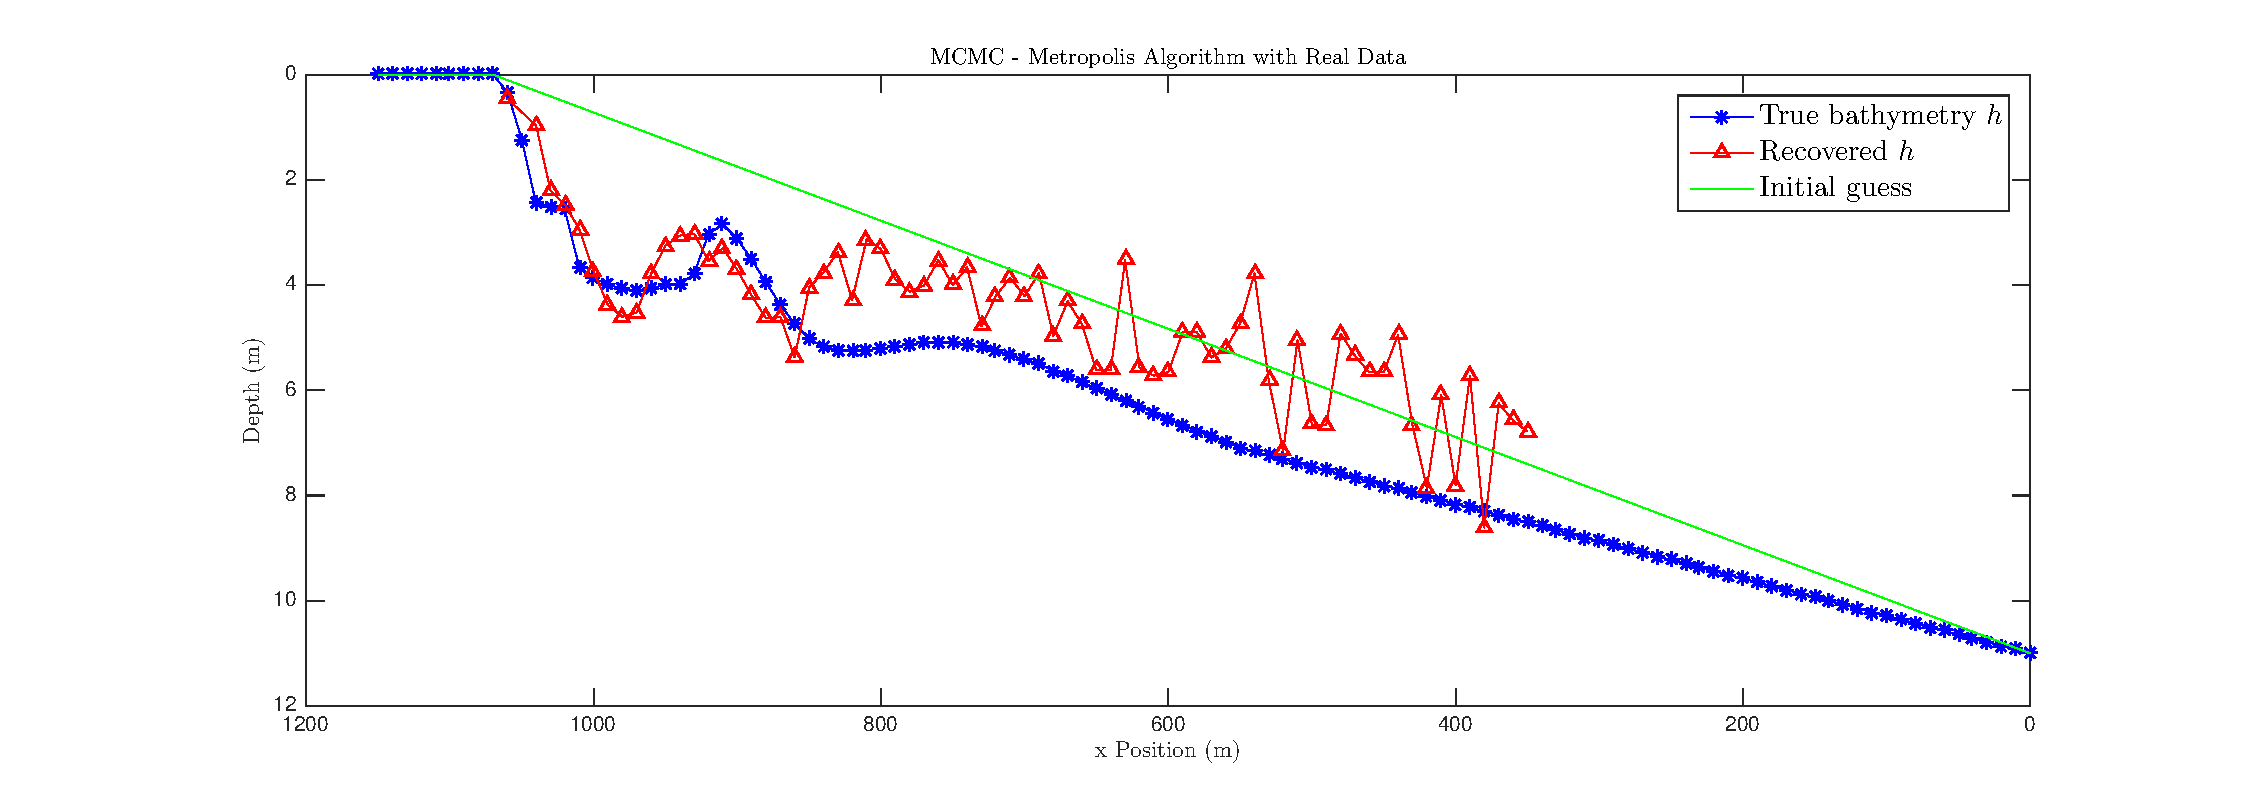
\includegraphics[scale=0.46]{img/MCMC-realdata-600.eps}
\caption{Bathymetry estimate from the Bayesian Markov Chain Monte Carlo (MCMC) approach using measured wave numbers as the objective in the likelihood function. The initial depth is shown in green, the true depth is shown in blue, and the derived estimate of depth is shown in red.}
\label{mcmc-real}
\end{figure}

Real $\mathbf{k}_m$ data is used to estimate the same bathymetry profile (see Figure~\ref{mcmc-real}). As with the synthetic case, we found a good match to the sandbar region around x position$\sim900~m$. However, the estimated depth decreases just seaward of the sand bar and does not correlate well with the true bathymetry for the remainder of the seaward domain. We expect the noisy spike in $\mathbf{k}$ seaward of the sandbar seen in  Figure~\ref{effectivewavenumbernoise} may be responsible for errors in our estimate of bathymetry in this area. The same issue occurs in the other inversion depth estimates. Note the real observed wave numbers are unavailable seaward of $\sim350~m$, so we do not estimate a depth for this region. 

Overall, the MCMC result performs better for the synthetic case, as may be expected given increased noise in real observations of $\mathbf{k}_m$. We compute this depth estimate using 1000 iterations with 250 burn in iterations and a proposal step size of 0.1. It it possible that inclusion of the wave height, $H$, as an additional objective in the likelihood function would improve estimates seaward of the sandbar where  wave number becomes less sensitive to depth, $h$, however we have yet to test this with the MCMC method. We also expect that additional scrutiny of our choices for the prior, proposal step size, and number of iterations could result in an improved bathymetry estimate given observed wave number, $\mathbf{k}_m$. 

\subsubsection{Posterior Probability Distributions}


Unlike the other methods, the Bayesian approach results in a distribution of depth profiles which optimize bathymetry given uncertain wave number. Measurements of wave number, $\mathbf{k}_m$, are not perfect and our resulting distribution of depth profiles translates that uncertainty into an ensemble of depth estimates which are consistent with the $\mathbf{k}_m$ data to within uncertainty. Figures~\ref{mcmc-posterior-h-synthetic} and \ref{mcmc-posterior-h-real} show the resulting posterior depth distributions. 

As expected, the posterior distribution shows confidence in the location and shape of the true bathymetry in the area of the sandbar. However, the posterior also seems to show confidence in the high variability area seaward of the sandbar. As discussed previously, we expect our estimates to perform poorly in the offshore region, which would suggest our posterior distribution demonstrate less confidence in this area. Further tests are needed to thoroughly examine this issue, but it is possible our Metropolis algorithm is heavily dependent on choices of the prior distribution and proposal function. 


\begin{figure}[H]
\center
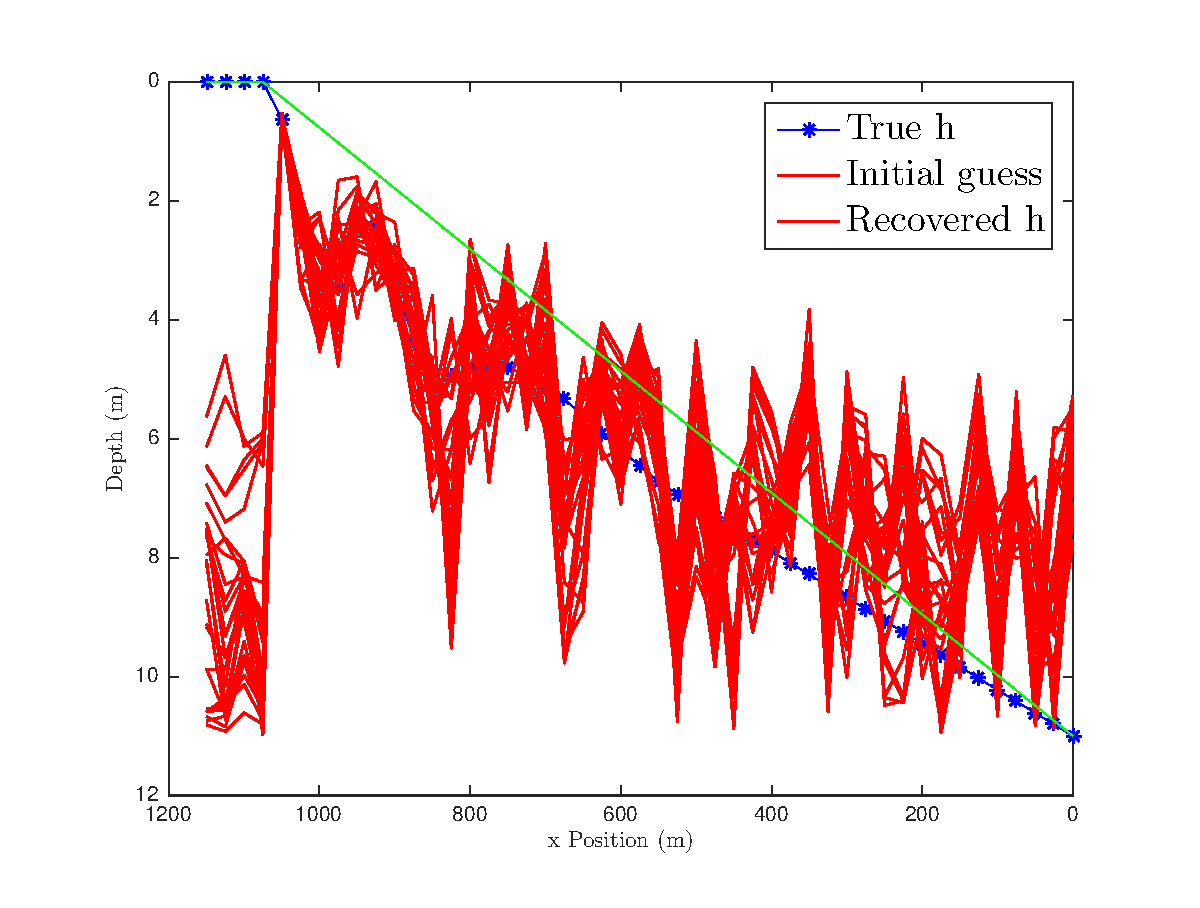
\includegraphics[scale=0.46]{img/MCMC-posterior-manufactured}
\caption{Posterior distribution of depth, $\mathbf{h}$, estimates for the manufactured data result. The distribution largely dithers around the result shown in Figure~\ref{mcmc-synthetic}. The posterior accurately predicts the location of the sandbar but appears to give false confidence to our bathymetry estimate elsewhere.}
\label{mcmc-posterior-h-synthetic}
\end{figure}


The posterior distribution resulting from use of real $k$ values leaves the position of the sandbar ambiguous because the posterior distribution does not appear to converge to a single solution. This suggests less confidence in our estimate of the sandbar bathymetry, though the maximum of our posterior density appears to converge to the true sandbar location. The lack of confidence in the real versus manufactured data results may be due to discrepancies in the number of iterations for each. Because the real data result is derived from only 1000 iterations as opposed to 20,000 for the manufactured data result, it is possible the solution has not converged sufficiently to the true posterior disribution of depth, $h$. Increasing the number of iterations and burn in may therefore improve the posterior distribution and therefore confidence in our estimate of the true bathymetry. 

